%!/usr/bin/env latex
% espina-user-manual.tex: EspINA user manual
% @Author:      <Jorge Peña> (<jpena@cesvima.upm.es>)
% @Created:     2012-09-17.
% @Last Change: 2012-09-17.
% @Revision:    0.0

\documentclass[a4paper,10pt]{article}

\usepackage{ifpdf}
\usepackage{ifthen}

% D E F I N I C I O N   D E   L A S   C A B E C E R A S   D E   C A P I T U L O S
\usepackage{type1cm}
\usepackage{floatflt}
\usepackage{float}

\ifpdf
  \usepackage{color,graphicx}
  \usepackage[pdftex, % or dvips or dvipsone
  %------------- Backref Switch ---------------------------
  pagebackref,                     % or backref
  %------------- Color Links ------------------------------
  colorlinks=false, %true,
  linkcolor=black, %webbrown,            % defined below
  filecolor=black, %blue,
  citecolor=black, %green,
%------------- Doc Info ---------------------------------
  pdftitle={EspINA User Manual},
  pdfauthor={Jorge Pena Pastor},
  pdfsubject={Reconstruction},
  pdfkeywords={reconstruction, neuroscience, fib},
%------------ Doc View ----------------------------------
bookmarksopen=false
%pdfpagemode=UseOutlines %is the default, use ``None'' otherwise
%hypertexnames=false
]
{hyperref}
  
  %defined in manuscrit.tex
  %\graphicspath{                  % where are the figures?
  %       {pdf/}{jpg/}
  % }
\else
  \usepackage[pagebackref]{hyperref}
  \usepackage{graphicx}
  \usepackage{color}
  %defined in manuscrit.tex
  %\graphicspath{                  % where are the figures?
  %	 {ps/} 
  %}
\fi

\definecolor{MyDarkBlue}{rgb}{0,0.1,0.45}%0,0.08,0.45
\hypersetup{citecolor=MyDarkBlue}

% FONTS
\usepackage[english]{babel}
\usepackage[utf8]{inputenc}
\usepackage[T1]{fontenc}

% MULTICOLUMNS
\usepackage{multicol}

% TABLE
\usepackage{longtable}
\usepackage{supertabular}

% FIGURES
\usepackage{fancybox}
%\usepackage{psfrag} 
\usepackage{subfigure}

% ENUMERATES
\usepackage{mdwlist}


% MATHEMATICS
\usepackage{amsmath,amssymb}
\usepackage{amscd}
\usepackage{amsfonts}
\usepackage{array}
\usepackage{mathrsfs}
\usepackage{textcomp}
\usepackage{latexsym}

% GRAPHISM
\usepackage{graphics}
\usepackage{pst-text} %to place text along curves

% LIST ENVIRONMENTS
\usepackage{enumitem}

% B I B L I O G R A P H I E
\usepackage[colon]{natbib}
% Biblio grafía en el índice
\usepackage{tocbibind} 

% T A B L E   O F   C O N T E N T   F O R   A P P E N D I X
\usepackage{appendix}

% U R L
\usepackage{url}

% PAGE
\usepackage[headings]{fullpage}
\usepackage{placeins}

% C O L O R S
\definecolor{webbrown}{rgb}{.6,0,0}
\definecolor{gris55}{gray}{0.55}
\definecolor{bleu}{rgb}{0,0,0.5}

\ifpdf
  \graphicspath{                  % where are the figures?
	  {fig/}
}
\else
  \graphicspath{                  % where are the figures?
	  {fig/}
}
\fi

% C A B E C E R A S   M O L O N A S
\usepackage{fancyhdr}
\pagestyle{fancy}
\fancyhf{}
\fancyfoot[LO,LE]{
\includegraphics[scale=0.29]{logo-cajal}}
\fancyfoot[CO,CE]{\thepage}
\fancyfoot[RO,RE]{
\includegraphics[scale=0.1]{logo-cesvima}}
\fancyhead[LO,LE]{\textbf{EspINA}}
\fancyhead[RO,RE]{\textbf{Cajal Blue Brain Project}}
\renewcommand{\headrulewidth}{0.5pt}
\renewcommand{\footrulewidth}{0.5pt}

% avoid text going farther than the footer line
\addtolength{\footskip}{20pt}

\usepackage{lastpage}
\usepackage{a4wide} 
\usepackage{moreverb}
\usepackage{hangcaption}
\usepackage{listings}

% NOTAS 
\usepackage[tikz]{bclogo}

%Formulas
\newcommand{\ela}{\\ \nonumber}
%Variables
%%Prob
\newcommand{\desc}[3]{
\begin{tabular}{m{0.8cm} m{13cm}}
\includegraphics[width=0.7cm]{#2} & \textbf{#1}: #3
\end{tabular}
}

%%CONSTANTS
\newcommand{\espina}{EspINA}

%%Writing
\newcommand{\ToDo}[1]{\textit{\textbf{ToDo: } #1}}

%P O R T A D A
\author{Cajal Blue Brain \\ CeSViMa}

\title{\textbf{Esp}ina \textbf{I}nteractive \textbf{N}euron \textbf{A}nalizer}

\begin{document}

\maketitle \clearpage
\tableofcontents \clearpage
%\listoffigures %\clearpage\listoftables


\section{Introduction}

\espina{} is a tool for segmenting, editing and analyzing neuroscientific images acquired using microscopy.
The program is been developed by the CesViMa (Centro de Supercomputación y Visualización de Madrid)
for the Cajal Blue Brain Project.


\section{Menus}
\subsection{File menu}

\begin{itemize}
\item \textbf{Open:} Loads a file and initiates a new \espina{} session.
\item \textbf{Add:} Loads and adds a file to the current session.
\item \textbf{Save:} Saves current session data to a SEG file.
\end{itemize}

\subsection{Analysis menu}

\begin{itemize}
\item \textbf{Segmentation information:} Toggles visibility of the ``Segmentation Information'' widget.
\end{itemize}

\subsection{Edit menu}

\begin{itemize}
\item \textbf{Undo:} Undo the last action.
\item \textbf{Redo:} Redo the last action removed by the undo function.
\end{itemize}

\subsection{View menu}

\begin{itemize}
\item \textbf{Panels:} Toggles the visibility of the following widgets:
	\begin{itemize}
	\item \textbf{Channel Explorer}
	\item \textbf{Filter Explorer}
	\item \textbf{Segmentation Explorer}
	\item \textbf{Taxonomy Explorer}
	\end{itemize}
\item \textbf{Color by:} Colorizes segmentations using one of the following criteria:
	\begin{itemize}
	\item \textbf{Taxonomy}
	\item \textbf{User}
	\item \textbf{Segmentation Id}
	\end{itemize}
\item \textbf{Views:} Toggles the visibility of the following planar view widgets:
	\begin{itemize}
	\item \textbf{XY:} Axial view.
	\item \textbf{XZ:} Coronal view.
	\item \textbf{YZ:} Sagittal view.
	\end{itemize}
\item \textbf{Show ruler:} Toggles the visibility of the size ruler over the planar views. The size unit is nanometers.
\item \textbf{Show thumbnail:} Toggles the visibility of the zoom thumbnail over the planar views.
\item \textbf{Switch channel:} Switches active channel function between loaded channels.
\item \textbf{Fit to slices:} Toggles the use of slicing step. When active the slice movement step in the planar views is the defined value of the image (in nanometers).
When not active the planar view allows free movement up to one nanometer in resolution.
\end{itemize}

\subsection{Settings menu}

\begin{itemize}
\item \textbf{Configure \espina:} Shows \espina{} configuration dialog.
\item \textbf{About:} Shows \espina{} about dialog.
\end{itemize}

\begin{bclogo}[couleur = yellow!33, logo=\bcattention]
{Note} Plugins can add items to menus. Refer to the plugin documentation for information.
\end{bclogo}


\section{\espina{} views}

\espina{} has two different types of view to represent the loaded images: a planar, 
two-dimensional view and a three-dimensional view. By default the program shows three
planar views (which correspond to the axial, coronal and sagittal views) and one
three-dimensional view. \\
Although both are interactive all work (segmentation, editing and analysis) is
performed in the planar view, leaving the three-dimensional view solely for
a three-dimensional representation of the results. \\
Both type of views can be docked into the main \espina{} window or can become floating
widgets if the user click and drags in the view title to it's new position. And can become
docked widgets if the user drags it back to the \espina{} main window. \\

\subsection{Two-dimensional view}

The two-dimensional views are formed by a view area and a slider bar. The view area is
used to operate with the channel or segmentations, and the slider is used to move through
the stack of images in the direction of the view. Alternatively you can use the mouse wheel
to get the same result as using the slider.\\

\begin{figure}[H]
\centering
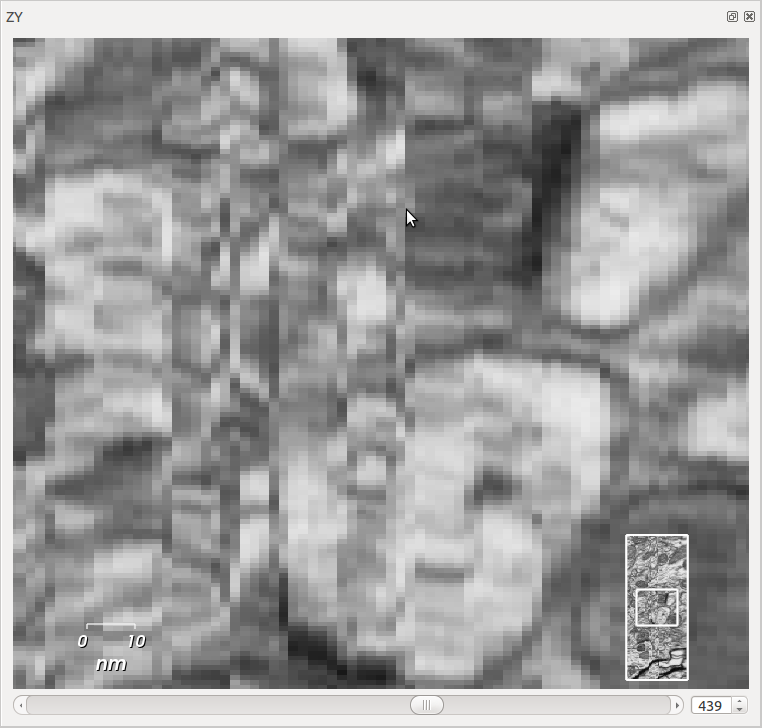
\includegraphics[scale=0.33]{fig/2DView}
\caption{Two-dimensional view, with thumbnail and ruler.}
\end{figure}

When there is no tool or widget in use the user can select a segmentation by left clicking
on it, or select a group of segmentations if the shift key is holded down while left clicking.\\
To move over the plane the user must click and hold the middle button of the mouse and move
the mouse in the direction he wants to translate the plane. To zoom the image, the operation is
similar to he previous one, but with the right button of the mouse. \\
Over the view area there can be two additional items: the size ruler, that gives us a measure of
size and distance, and the slice thumbnail, that appears when the image is too big to completely
fit into the view area and shows us the part of the slice we are looking at. Movement over the
plane is also possible left clicking on the thumbnail when it's present.

\subsection{Three-dimensional view}

The three-dimensional view is formed by a view area and a set of buttons on the right and 
left of the bottom of the view. \\
As noted before, the three dimensional view shows a interactive representation of the
segmentations and other data like, for example, the crosshair position.\\
The operation of the three-dimensional view is similar to what was explained in the previous
subsection for the planar view. Translating and zooming works the same way (with the exception
that now the mouse wheel can be also used to zoom the scene), and to rotate the representation
the user must hold down the left mouse button and move it in the direction he wants to rotate.\\

\begin{figure}[H]
\centering
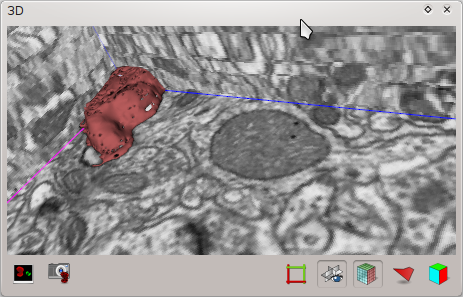
\includegraphics{fig/VolumeView}
\caption{Three-dimensional view widget.}
\end{figure}

The buttons at the bottom-left of the view allows the user to export the representations as a image
or a three-dimensional scene.\\
\vspace{0.2cm}

\begin{tabular}{| m{1.3cm} | m{12cm} |}
\hline
\textbf{Button} & \textbf{Description}\\
\hline

\includegraphics[width=0.7cm]{../../frontend/rsc/snapshot_scene} & 
\textbf{Take Snapshot}: Save an snapshot of the current view. Supported formats:
\begin{itemize}
\item JPG (Joint Photographic Experts Group)
\item PNG (Portable Network Graphics)
\end{itemize}\\
\hline

\includegraphics[width=0.7cm]{../../frontend/rsc/export_scene} &
\textbf{Export 3D Scene}: Export current displayed scene into a 3D compatible format. Supported formats:
\begin{itemize}
\item POV (Persistence Of Vison)
\item VRML (Virtual Reality Modelling Languange)
\item X3D (XML-based format, the successor of VRML)
\end{itemize}
\begin{bclogo}[couleur = yellow!33, logo=\bcattention]
{Note} Only the mesh objects of the scene are exported, volumetric objects are not. This is a limitation of the destination formats.
\end{bclogo}\\
\hline
\end{tabular}
\vspace{0.3cm} 

On the bottom-right there is the set of buttons called ``renderers''. A renderer is
a way to represent information that can be toggled (activated or deactivated). By
default \espina{} shows three renderers.

\begin{tabular}{| m{1.3cm} | m{12cm} |}
\hline
\textbf{Button} & \textbf{Description}\\
\hline

\includegraphics[width=0.7cm]{../../frontend/rsc/show_planes} &
\textbf{Crosshair Renderer}: Toggle channel's crosshair planes visibility.\\
\hline
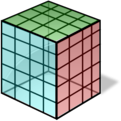
\includegraphics[width=0.7cm]{../../frontend/rsc/mesh} &
\textbf{Mesh Renderer}: Toggle segmentation's mesh rendering.\\
\hline
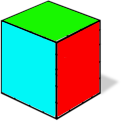
\includegraphics[width=0.7cm]{../../frontend/rsc/voxel} &
\textbf{Volumetric Renderer}: Toggle segmentation's volumetric rendering.\\
\hline
\end{tabular}
\vspace{0.3cm} 

Additionally plugins can add buttons to this set of renderers. Refer to the plugin
documentation for a description of those.



\section{User Interface}

\subsection{General Purpose Tools}
\begin{figure}[H]
\centering

\includegraphics[scale=0.65]{fig/MainToolbar}
\caption{General purpose toolbar.}
\end{figure}

These tools offer basic funcionality independent of any specific context.\\

\vspace{0.3cm}
%\desc{Show Segmentations}{../../frontend/rsc/show_all}
%{Segmentations are shown in planar views}
\begin{tabular}{| m{1.3cm} | m{12cm} |}
\hline
\textbf{Button} & \textbf{Description}\\
\hline
& Visibility button is a toggle button with two states.\\ 

\includegraphics[width=0.6cm]{../../frontend/rsc/show_all} &
\textbf{Show Segmentations}: All segmentations are shown in planar views.\\

\includegraphics[width=0.6cm]{../../frontend/rsc/hide_all} &
\textbf{Hide Segmentations}: All segmentations are hidden in planar views.\\
\hline
& Crosshair button is a toggle button with two states.\\ 

\includegraphics[width=0.6cm]{../../frontend/rsc/show_planes} &
\textbf{Show Crosshair}: Crosshair is shown in planar views.\\
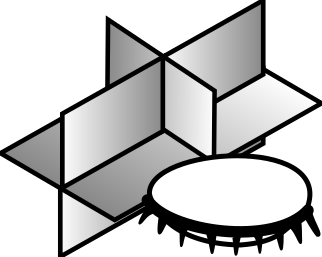
\includegraphics[width=0.6cm]{../../frontend/rsc/hide_planes} &
\textbf{Hide Crosshair}: Crosshair is hidden in planar views.\\
\hline
 & %No icon
\textbf{Taxonomy Selector}: Some tools may require the user to specify a
taxonomy label to be applied when segmentations are created.\\
\hline

\includegraphics[width=0.6cm]{../../frontend/rsc/removeSeg} &
\textbf{Delete Segmentation}: Deletes segmentations by clicking on them on one of the planar views.\\
\hline
\end{tabular}

\subsection{Volume Of Interest}

It's a volume to limit the effect of other tools, so the tool algorithm will not
go farther than the boundaries that define the volume.\\

To use it, just click on the toolbar button an then left click on the center of
the view area you want to place the volume of interest. Once the volume has been
placed the user can modify it's dimensions by clicking and dragging on the edges.\\

Only a volume of interest can be applied at a given time.\\

\vspace{0.3cm}
\begin{tabular}{| m{1.3cm} | m{12cm} |}
\hline
\textbf{Button} & \textbf{Description}\\
\hline

\includegraphics[width=0.6cm]{../../frontend/toolbar/voi/rsc/roi} &
\textbf{Rectangular Cuboid}: Define an axis aligned rectangular cuboid as volume
of interest.\\
\hline
\end{tabular}

\subsection{Channel Explorer}
Display all channels, grouped by physical sample, that are currently
loaded.Channel visibility can be toggled by clicking on the \textit{eye} icon on
the left of channels.Certain \espina's tools may require selecting channel in
order to be used. These tools will use the active channel. Active channels are
displayed in bold font in Channel Explorer.

\begin{figure}[H]
\centering
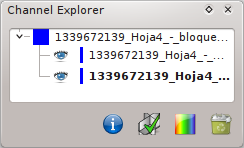
\includegraphics{fig/ChannelExplorer}
\caption{Channel explorer widget.}
\end{figure}

\begin{tabular}{| m{1.3cm} | m{12cm} |}
\hline
\textbf{Button} & \textbf{Description}\\
\hline
 & \textbf{Spacing Information}: Modify channel's spacing.\\
\hline

\includegraphics[width=0.6cm]{../../frontend/rsc/activeChannel} &
\textbf{Activate Channel}: Mark selected channel as active channel. Operations
are always applied to the active channel independently whether they are visible
or not.\\
\hline

\includegraphics[width=0.6cm]{../../frontend/rsc/rainbow} &
\textbf{Change Stain}: Display stain color selector for selected channel.\\
\hline

\includegraphics[width=0.6cm]{../../frontend/rsc/trash-full} &
\textbf{Unload Channel}: Unload current channel from \espina. The channel itself
is not modified nor deleted from disk.\\
\hline
\end{tabular}
\vspace{0.3cm}

\subsection{Taxonomy Explorer}
Display available taxonomy elements. Users can create new taxonomy's elements,
modify or delete existing ones.
\begin{figure}[H]
\centering
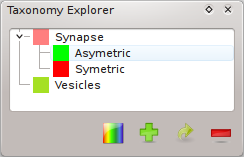
\includegraphics{fig/TaxonomyExplorer}
\caption{Taxonomy explorer widget.}
\end{figure}

\begin{tabular}{| m{1.3cm} | m{12cm} |}
\hline
\textbf{Button} & \textbf{Description}\\
\hline

\includegraphics[width=0.6cm]{../../frontend/rsc/rainbow} &
\textbf{Change Color}: Display a color selector window to change the color
assoicated with selected taxonomy.\\
\hline

\includegraphics[width=0.6cm]{../../frontend/rsc/create_node} &
\textbf{Add Taxonomy}: Create a new segmentation at the same level than the
selected one.\\
\hline

\includegraphics[width=0.6cm]{../../frontend/rsc/create_subnode} &
\textbf{Add SubTaxonomy}: Create a new segmentation as a child of the selected
one.\\
\hline

\includegraphics[width=0.6cm]{../../frontend/rsc/remove} &
\textbf{Delete Taxonomy}: Delete selected taxonomy. Only taxonomies which are
not in use can be deleted.\\
\hline
\end{tabular}
\vspace{0.3cm}

\subsection{Segmentation Explorer}
Display all segmentations that are currently loaded. Segmentation visibility can
be toggled by clicking on the \textit{eye} icon on the left of segmentations.
\begin{figure}[H]
\centering
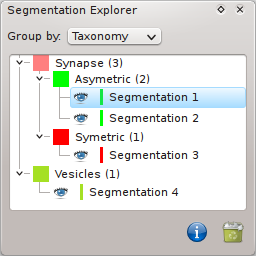
\includegraphics{fig/SegmentationExplorer}
\caption{Segmentation explorer widget.}
\end{figure}

Segmentations can be arranged using different grouping critearias:
\begin{itemize}
  \item None Display a list with all segmentations.
  \item Taxonomy Display each segmentation under their corresponding taxonomy
element.
  \item Sample Display each segmentation under their corresponding sample.
\end{itemize}
\vspace{0.3cm}

\begin{tabular}{| m{1.3cm} | m{12cm} |}
\hline
\textbf{Button} & \textbf{Description}\\
\hline
 & %No icon
\textbf{Segmentation Information}: Open the segmentation inspectors for the
selected segmentations.\\
\hline

\includegraphics[width=0.6cm]{../../frontend/rsc/trash-full} &
\textbf{Delete Segmentation}: Delete selected segmentations. When a grouping
element is selected, recursive deletion is available.\\
\hline
\end{tabular}
\vspace{0.3cm}

\subsubsection{Segmentation Inspector}
Display all available information of a segmentation. Available 3D
representations can be displayed using the three-dimensioanl view. Information
about the creation of the segmentation is displayed in the filter inspector on
the right side of the window. Finally, all available information is displayed
in the segementation information data table under the three-dimensional view.

\begin{figure}[H]
\centering
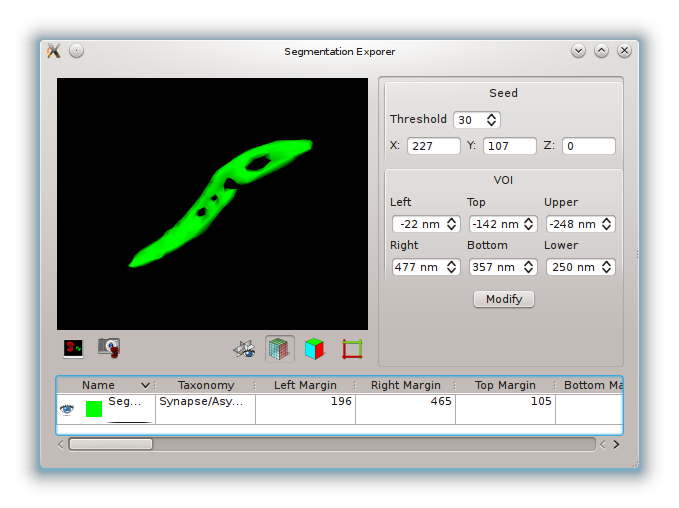
\includegraphics[width=\linewidth]{fig/SegmentationInspector}
\caption{Segmentation inspector widget.}
\end{figure}

For more specific information of each component, please refer to the
corresponding section.

\subsection{Filter Inspector}
The filter inspector shows relevant information about the filter that created the segmentation,
therefore the information shown is dependent on the filter or plugin filter used.

\begin{figure}[H]
\centering
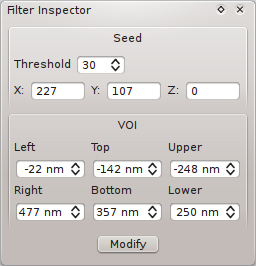
\includegraphics{fig/SeedGrowSegmentationFilterInspector}
\caption{Filter inspector widget showing the information of a seed grow filter.}
\end{figure}


\section{Using \espina}

\subsection{General Purpose Tools}
\begin{figure}[H]
\centering

\includegraphics[scale=0.75]{fig/MainToolbar}
\caption{General purpose toolbar.}
\end{figure}

%\desc{Show Segmentations}{../../frontend/rsc/show_all}
%{Segmentations are shown in planar views}
\begin{tabular}{| m{1.3cm} | m{12cm} |}
\hline
\textbf{Button} & \textbf{Description}\\
\hline
& Visibility button is a toggle button with two states.\\ 

\includegraphics[width=0.7cm]{../../frontend/rsc/show_all} &
\textbf{Show Segmentations}: All segmentations are shown in planar views.\\

\includegraphics[width=0.7cm]{../../frontend/rsc/hide_all} &
\textbf{Hide Segmentations}: All segmentations are hidden in planar views.\\
\hline
& Crosshair button is a toggle button with two states.\\ 

\includegraphics[width=0.7cm]{../../frontend/rsc/show_planes} &
\textbf{Show Crosshair}: Crosshair is shown in planar views.\\
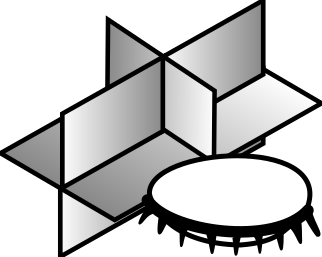
\includegraphics[width=0.7cm]{../../frontend/rsc/hide_planes} &
\textbf{Hide Crosshair}: Crosshair is hidden in planar views.\\
\hline
 & %No icon
\textbf{Taxonomy Selector}: Some tools may require the user to specify a
taxonomy label to be applied when segmentations are created.\\
\hline

\includegraphics[width=0.7cm]{../../frontend/rsc/removeSeg} &
\textbf{Delete Segmentation}: Deletes segmentations by clicking on them on one of the planar views.\\
\hline
\end{tabular}

\subsection{Channel Explorer}
Allows the user to individually toggle the visibility of each channel using a toogle button
located next to the channel's name whose function is similar of that described in the
general-purpose tools section.

\begin{figure}[H]
\centering
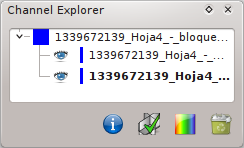
\includegraphics{fig/ChannelExplorer}
\caption{Channel explorer widget.}
\end{figure}

\begin{tabular}{| m{1.3cm} | m{12cm} |}
\hline
\textbf{Button} & \textbf{Description}\\
\hline
 & \textbf{Spacing Information}: Modify channel's spacing.\\
\hline

\includegraphics[width=0.7cm]{../../frontend/rsc/activeChannel} &
\textbf{Activate Channel}: Mark selected channel as active channel. Operations
are always applied to the active channel independently whether they are visible
or not.\\
\hline

\includegraphics[width=0.7cm]{../../frontend/rsc/rainbow} &
\textbf{Change Stain}: Display stain color selector for selected channel.\\
\hline

\includegraphics[width=0.7cm]{../../frontend/rsc/trash-full} &
\textbf{Unload Channel}: Unload current channel from \espina. The channel itself
is not modified nor deleted from disk.\\
\hline
\end{tabular}
\vspace{0.3cm}

\subsection{Taxonomy Explorer}

\begin{figure}[H]
\centering
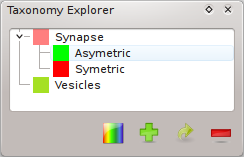
\includegraphics{fig/TaxonomyExplorer}
\caption{Taxonomy explorer widget.}
\end{figure}

\begin{tabular}{| m{1.3cm} | m{12cm} |}
\hline
\textbf{Button} & \textbf{Description}\\
\hline

\includegraphics[width=0.7cm]{../../frontend/rsc/rainbow} &
\textbf{Change Color}: Display taxonomy color selector for selected taxonomy.\\
\hline

\includegraphics[width=0.7cm]{../../frontend/rsc/create_node} &
\textbf{Add Taxonomy}: Create a new segmentation at the same level than the
selected one.\\
\hline

\includegraphics[width=0.7cm]{../../frontend/rsc/create_subnode} &
\textbf{Add SubTaxonomy}: Create a new segmentation as a child of the selected
one.\\
\hline

\includegraphics[width=0.7cm]{../../frontend/rsc/remove} &
\textbf{Delete Taxonomy}: Delete selected taxonomy.\\
\hline
\end{tabular}
\vspace{0.3cm}

\subsection{Segmentation Explorer}
Allows the user to individually toggle the visibility of each segmentation using a toogle button
located next to the segmentation's name whose function is similar of that described in the
general-purpose tools section.
\begin{figure}[H]
\centering
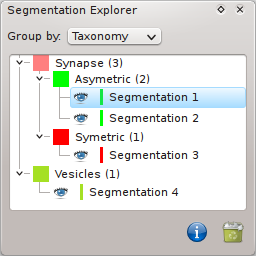
\includegraphics{fig/SegmentationExplorer}
\caption{Segmentation explorer widget.}
\end{figure}

\begin{tabular}{| m{1.3cm} | m{12cm} |}
\hline
\textbf{Button} & \textbf{Description}\\
\hline
 & %No icon
\textbf{Segmentation Information}: Open the segmentation inspectors for the
selected segmentations.\\
\hline

\includegraphics[width=0.7cm]{../../frontend/rsc/trash-full} &
\textbf{Delete Segmentation}: Delete selected segmentations.\\
\hline
\end{tabular}
\vspace{0.3cm}

\subsubsection{Segmentation Inspector}

Window composed of several widgets:
\begin{itemize}
\item a three-dimensional view
\item a filter inspector 
\item a data view
\end{itemize}
These widgets contain information about a single segmentation.

\begin{figure}[H]
\centering
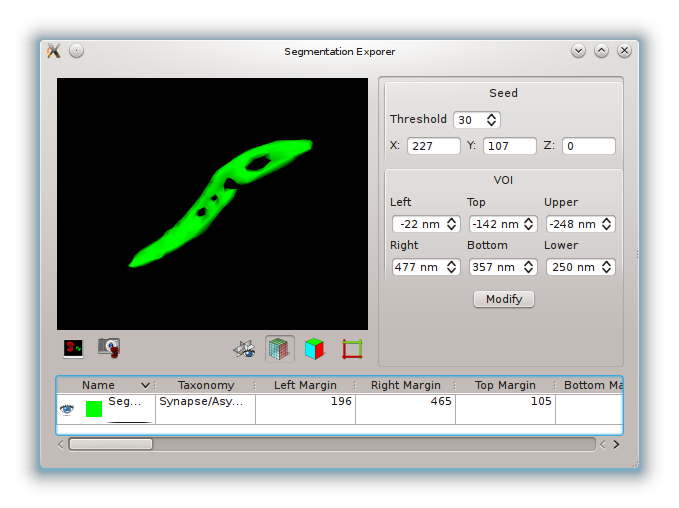
\includegraphics[width=\linewidth]{fig/SegmentationInspector}
\caption{Segmentation inspector widget.}
\end{figure}

For more specific information, please refer to the corresponding section.

\subsection{Volume Of Interest}

It's a volume to limit the effect of other tools, so the tool algorithm will not
go farther than the boundaries that define the volume.\\
To use it, just click on the toolbar button an then left click on the center of
the view area you want to place the volume of interest. Once the volume has been
placed the user can modify it's dimensions by clicking and dragging on the edges.\\
The user can define no more than one volume of interest at a given time. 

\vspace{0.3cm}
\begin{tabular}{| m{1.3cm} | m{12cm} |}
\hline
\textbf{Button} & \textbf{Description}\\
\hline

\includegraphics[width=0.7cm]{../../frontend/toolbar/voi/rsc/roi} &
\textbf{Rectangular Cuboid}: Define an axis aligned rectangular cuboid as volume
of interest.\\
\hline
\end{tabular}


\subsection{Seed Grow Segmentation}

This tool provides a semi-automated segmentation algorithm. Select a voxel
belonging to the object being segmented. A new segmentation will be createad
including all voxel which are equivalent (in gray scale values) to the selected
one, the seed.\\
If you have defined your own ``volume of interest'', then that is used instead of
the default one when applying the algorithm. The volume of interest will limit the
effect of the algorithm to the space enclosed within the volume.\\

\begin{figure}[H]
\centering
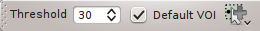
\includegraphics{fig/SeedGrowSegmentation}
\caption{Seed grow toolbar.}
\end{figure}
\vspace{0.3cm}

\begin{tabular}{| m{1.3cm} | m{12cm} |}
\hline
\textbf{Button} & \textbf{Description}\\
\hline
& %No icon
\textbf{Threshold}: Gray scale difference admisible to consider a voxel equal to
the one selected as seed. \\
\hline
& %No icon
\textbf{Default VOI}: Determine whether or not a rectangular volume of interest
centered on the selection point is applied.\\
\hline
\includegraphics[width=0.7cm]{../../frontend/toolbar/seedgrow/rsc/pixelSelector} &
\textbf{Pixel Selector}: Create a new segmentation using the voxel under the
cursor as seed for the Seed Grow Algorithm.\\
\hline
\includegraphics[width=0.7cm]{../../frontend/toolbar/seedgrow/rsc/bestPixelSelector} &
\textbf{Best Pixel Selector}: Create a new segmentation using the best voxel
,within the neighborhood of the voxel under the cursor, as seed for the Seed
Grow Algorithm. \\
\hline
\end{tabular}

\vspace{0.3cm}
\begin{bclogo}[couleur = yellow!33, logo= \bcbook]
{Tip} Use Ctrl+Wheel to change threshold while any selector is active. 
\end{bclogo}
\vspace{0.3cm}

Best voxel is defined in terms of gray scale similarity with a
reference gray scale value. The reference value can be configured at Seed Grow
Segmentation settings panel.\\

\subsubsection{Filter Inspector}
The filter inspector shows relevant information about the filter that created the segmentation,
therefore the information shown is dependent on the filter or plugin filter used.

\begin{figure}[H]
\centering
\includegraphics{fig/SeedGrowSegmentationFilterInspector}
\caption{Filter inspector widget showing the information of a seed grow filter.}
\end{figure}



\section{Edition}

Segmentation tools, even if they are semi-automatic, need to be retouched in order to improve some analitical results.


\section{Analysis}




\section{Global shortcuts}

If \espina{} is not using a tool or a widget that modifies keyboard behaviour then the following keyboard shortcuts are available to the user:
\begin{itemize}
\item \textbf{Control key + left mouse click:} Changes crosshair position.
\item \textbf{Control key + space key:} Switches active channel function between loaded channels.
\item \textbf{Control key + Z key:} Undo last action.
\item \textbf{Control key + Shift key + Z key:} Redo last removed undo action.
\item \textbf{C key:} Toggle Crosshair visibility.
\item \textbf{Space key:} Toggle segmentations visibility.

\end{itemize}



\section{Configuration}

\subsection{General}

The general configuration allows the user to enter a identification. Also the user can specify where will the program store the auto save files and how often will the program backup the ongoing session.

\begin{figure}[H]
\centering
\includegraphics[scale=0.75]{fig/Configuration-general}
\caption{General configuration widget.}
\end{figure}

\subsection{View}

The view configuration offer the posibility of inverting the slice order in each of the planar views, reversing the stack only for that view, and to invert the use of the mouse wheel. \\
For the three-dimensional view, the renderers can be marked as active (meaning the three-dimensional view will add a button to enable/disable that representations) or available (won't appear on the renderers list in the 3D view widget).
\vspace{0.3cm}
\begin{bclogo}[couleur = yellow!33, logo=\bcattention]
{Note} Plugins can add their own renderers. Refer to the plugin documentation for more information.
When a renderer is added it is by default marked as ``Available''.
\end{bclogo}

\begin{figure}[H]
\centering
\includegraphics[scale=0.75]{fig/Configuration-view}
\caption{View configuration widget.}
\end{figure}

\subsection{Seed grow segmentation}

The value of the ``best pixel'' used in the seed grow segmentation algorithm can be configured using a slider bar that goes from a complete black value to a complete white one. Also the size of the ``volume of interest'' can be defined by giving the length of each of it's sides.\\
Once the seed algorithm has obtained a segmentation usually the user applies a closing algorithm to make it compact. The option to make this step automatic can be configured here, with the possibility of specifying the radious of the structuring element of the closing algorithm. 

\begin{figure}[H]
\centering
\includegraphics[scale=0.75]{fig/Configuration-seed}
\caption{Seed grow segmentation configuration widget.}
\end{figure}

\subsection{Edition tools}

The radious of the paint and erase brushes can be configured in screen pixels. Also the structuring element radious of the morphological filters can be modified. 

\begin{figure}[H]
\centering
\includegraphics[scale=0.65]{fig/Configuration-edit}
\caption{Edition tools configuration widget.}
\end{figure}




\section{Plugins}

A plugin is a way of extending \espina{} functionality. It can
add a new element to the program, be it a new renderer, widget or
extension. \\
This section will document just the plugins included with \espina.

\subsection{Apposition Surface Plugin}

An apposition plane is the planar surface that best fit the structure of a
segmentation.\\

\vspace{0.3cm}

\desc{Show Apposition Surface}{../../frontend/rsc/appPlane}
{Display segmentation's apposition surface}


\subsection{Counting Region plugin}

A ``counting region'' is a volume for counting synapses. The boundaries of this
volume are marked red or green, indicating that a synapse touching the green boundary
will be marked as inside the volume and will be counted. On the other side a synapse
touching the red boundary wont be counted. Obviously the synapses inside of the volume
will be counted and the ones outside won't.\\
\espina{} will allow the existance of various regions for counting, each of one will
define it's own exclusion and inclusion boundaries.\\
This plugin will add representations to the corresponding planar views and will add a 
renderer to the three-dimanensional view. A widget will be added to the main widgets list 
so the user can create, modify and define the type of region.\\

\begin{figure}[H]
\centering
\includegraphics[scale=0.5]{fig/plugin-ct-2Dwidget.png}
\caption{Two-dimensional view showing one counting region boundaries for this view.}
\end{figure}

The two-dimensional representations will allow the user to modify the definition of the
boundaries by left-clicking and dragging them around, while the three-dimensional
representation will just show these boundaries.\\

\begin{figure}[H]
\centering
\includegraphics[scale=0.5]{fig/plugin-ct-widget.png}
\caption{Counting Region widget.}
\end{figure}

The counting region widget allow the user to manually edit the type and boundaries of several
counting regions.\\

\begin{tabular}{| m{1.3cm} | m{12cm} |}
\hline
\textbf{Button} & \textbf{Description}\\
\hline
Margins & Manually set left, right, top, bottom, upper and lower margins.\\
\hline
Type & Defines the type of the region.\\
\hline
\includegraphics[width=0.7cm]{../../plugins/CountingRegion/rsc/apply} & Creates a new region of the selected type.\\
\hline
\includegraphics[width=0.7cm]{../../plugins/CountingRegion/rsc/trash-full} & Deletes the region selected in the region selection list.\\
\hline
Selection list & Selection box shows the margins and type of the region.\\
\hline
Region description & Lists the properties of the region.\\
\hline
\end{tabular}
\vspace{0.3cm} 

A counting region can be defined as:
\begin{itemize}
\item \textbf{Rectangular:} The region volume is largest possible parallelogram that encloses all the slices.
\item \textbf{Adaptative:} The region volume is the smallest possible, adapting it's boundaries to every slice.
\end{itemize}


\subsection{Tubular Segmentation plugin}

This plugin adds a new interactive way of defining segmentations. The user creates a
segmentation by defining a list of spheres (centers and radious) in the three-dimensional
space of the sample, that will be later connected with tubes.
That way a tubular segmentation is created.\\

\begin{figure}[H]
\centering
\includegraphics[scale=0.2]{fig/plugin-ts-segmentation.png}
\caption{A tubular segmentation with flat extremes.}
\end{figure}

To create a tubular segmentation use the associated toolbar. The toolbar is used to \textbf{create} a
new segmentation. To \textbf{modify} an existing segmentation the user must use a similar button located
in the filter inspector.
 
\begin{figure}[H]
\centering
\includegraphics[scale=0.75]{fig/plugin-ts-toolbar.png}
\caption{Tubular segmentations toolbar.}
\end{figure}

\begin{tabular}{| m{1.3cm} | m{12cm} |}
\hline
\textbf{Button} & \textbf{Description}\\
\hline
\includegraphics[width=0.7cm]{fig/tubular} & Create a new tubular segmentation.\\
\hline
\end{tabular}
\vspace{0.3cm} 

To create a segmentation the user must click on the screen to define a sphere centen and, once the center
has been defined, a sphere border will be created. The user must then define the length of the radius of the 
sphere by clicking on the screen again when it has reached the desired lenght. To place the next sphere in
the tubular segmentation the user must repeat the process used to create the first. When the next sphere has
been defined the interface will show the tube that joins both spheres, and so on. \\
By default the newly created segmentation won't have it's extremes rounded, that is shown during creation by
drawing the first and last spheres with a discontinuous border, while the rest of the spheres will have a
solid border. This behaviour can be changed in the filter inspector. \\

In the filter inspector widget of a tubular segmentation the nodes that define the segmentation are shown.\\

\begin{figure}[H]
\centering
\includegraphics[scale=0.75]{fig/plugin-ts-inspector.png}
\caption{Tubular segmentations toolbar.}
\end{figure}

\begin{tabular}{| m{1.3cm} | m{12cm} |}
\hline
\textbf{Button} & \textbf{Description}\\
\hline
Nodes & Node list with the coordinates of the center of the node and it's radius.\\
\hline
\includegraphics[width=0.7cm]{fig/tubular} & Modify the nodes that define this segmentation.\\
\hline
Save & Save the node list to a text file.\\
\hline
Round Extremes & Toggles between rounded/flat extremes segmentations.\\
\hline
\end{tabular}
\vspace{0.3cm} 





%\bibliographystyle{alpha}
%\bibliography{rapport-mosig}

%\newpage

%\appendix

%\input{variables.tex}

%\input{architecture.tex}

%\input{coax_environment.tex}


\end{document}
